%=======================================================================
% Declarações iniciais identificando a classe de documento e
% selecionando alguns pacotes adicionais.
%
% As opções disponíveis (separe-as com vírgulas, sem espaço) são:
% - twoside: Formata o documento para impressão frente-e-verso
%   (o default é somente-frente)
% - english,brazilian,french,german,etc.: idiomas usados no documento.
%   Deve ser colocado por último o idioma principal.
%=======================================================================
\documentclass[twoside,english,brazilian]{UNISINOSartigo}
\usepackage[utf8]{inputenc} % charset do texto (utf8, latin1, etc.)
\usepackage[T1]{fontenc} % encoding da fonte (afeta a sep. de sílabas)
\usepackage{graphicx} % comandos para gráficos e inclusão de figuras
\usepackage{bibentry} % para inserir refs. bib. no meio do texto
\usepackage{placeins}

\usepackage{adjustbox}

\unisinosbst

%================================================================
% Início do documento.
%================================================================
\begin{document}
\titulo{Insight: Um modelo acessível para localização em ambientes internos usando a tecnologia Bluetooth Low Energy}
\autor{Paulo Henrique Grolli Gräbin\footnote{Aluno do curso de Ciência da Computação.  Email: paulograbin@gmail.com}}
\autor{Cristiano André da Costa\footnote{Orientador, professor da Unisinos, doutor em Ciência da Computação pela Universidade Federal do Rio Grande do Sul (2008), Mestre em Ciência da Computação pela mesma Universidade (1997). Email: cac@unisinos.br}}

%=======================================================================
% Resumo em Português.
%=======================================================================
\begin{abstract}
Deficientes visuais passam por grandes dificuldades durante seu deslocamento, devido ao fato de não poderem contar com a sinalização visual, que frequentemente é a única disponível. Aliado a isso, sistemas de posicionamento comumente fazem uso da tecnologia GPS, que se prova insuficiente em ambientes internos. Visando mitigar esse problema, este trabalho tem como objetivo descrever um modelo computacional denominado Insight. O Insight foi desenvolvido para ser utilizado por pessoas com deficiência visual, fornecendo uma localização confiável e um deslocamento seguro através de instruções de voz, leitura de tela e feedback tátil, permitindo que seus usuários possam se deslocar em ambientes desconhecidos sem a necessidade de auxílio de outras pessoas. O modelo é baseado em uma estrutura de serviço na nuvem, contando com servidores distribuídos, onde os clientes são dispositivos móveis que contemplam diversas formas de interação, afim de possibilitar da forma mais natural possível a integração do sistema com a vida diária do usuário. Para a avaliação, foi usada a metodologia de cenários, na qual foram criados dois cenários para testar a viabilidade do modelo e o seu comportamento em um ambiente que simula a rotina de uma pessoa com deficiência visual.

\palavraschave{Acessibilidade Ubíqua\@.  Deficiência Visual\@.  Sistemas de Posicionamento Indoor.}
\end{abstract}

%=======================================================================
% Introdução
%=======================================================================
\section{Introdução}
A visão é o recurso mais importante na localização de um indivíduo e na percepção do que se passa ao seu redor. Frequentemente, a sinalização destinada a orientação em locais como aeroportos, shopping centers e universidades é composta inteiramente por sinais visuais. Por esse motivo, pessoas com deficiência visual (PDV) tem grande dificuldade quando necessitam se deslocar, precisando do auxílio de ferramentas como bengalas e cães-guia ou ainda da ajuda de outras pessoas.

De acordo com o levantado por \citetexto{IBGE2010}, no último Censo Demográfico, realizado em 2010, o Brasil possuía 45,6 milhões de pessoas que afirmaram ser portadoras de deficiência. Desse total, 35,7 milhões, ou 78,2\%, são pessoas com deficiência visual (PDV). Ou seja, aproximadamente 18\% da população brasileira é afetada.

Em 2014, a Royal London Society for Blind People (RLSB), organização sem fins lucrativos que busca criar uma diferença que melhore a vida das futuras gerações de PDV, divulgou um manifesto para chamar atenção aos desafios enfrentados diariamente pelos PDV, que os impedem de usufruir da totalidade dos seus direitos fundamentais. \cite{YouthManifesto}. Desafios esses que não são restritos às divisas do Reino Unido, onde a organização se encontra.
De acordo com o documento, perda de visão é uma experiência tão traumática que pode ser comparada à perda de um ente querido, visto que dificilmente eles recebem o apoio emocional necessário. Não conseguir enxergar causa isolamento social, o que prejudica enormemente o futuro do indivíduo. Ainda é dito que empresas ou organizações, como lojas, bancos e agentes de viagem, não compreendem as necessidades e habilidades dos PDV, impedindo-os de levar uma vida comum e impossibilitando-os de realizar as atividades que gostariam. O trabalho ainda destaca que, frequentemente, as pessoas não sabem oferecer assistência básica, como guiá-los em espaços públicos, estações de trem, por exemplo. Dentre as áreas citadas como problemáticas, é possível destacar a mobilidade urbana, a educação superior e acessibilidade na tecnologia. No trabalho ainda é revelado o motivo de sua publicação, informando que 25\% das pessoas com perda de visão estão insatisfeitas com suas vidas. \cite{YouthManifesto}.

Em relação à mobilidade, \citetexto{YouthManifesto} cita que existe uma variedade de aplicativos para smartphone que auxiliam pessoas a se localizar e se deslocar, porém, poucos deles são acessíveis. É afirmado também que, se essas tecnologias fossem projetadas com todas as pessoas em mente, mais PDV poderiam transitar com segurança, reduzindo a dependência de outras pessoas.

Indo ao encontro das iniciativas das RLSB e atuando na área de mobilidade, o presente trabalho apresenta um modelo que faz uso de conceitos como dispositivos móveis, acessibilidade ubíqua, tecnologias assistivas e localização por Bluetooth Low Energy (BLE). O modelo trata de uma alternativa para facilitar as atividades diárias das pessoas com deficiência, especialmente a visual, atuando na forma com que elas se orientam e se deslocam em ambientes internos.

Tendo a premissa de funcionar a partir do smartphone do usuário, o sistema irá informar ao usuário sua localização atual e recomendar caminhos que o levem ao seu destino, levando em consideração os obstáculos em sua rota. O sistema será projetado para ter usabilidade intuitiva e ser uma parte quase invisível do cotidiano do usuário, aplicando o conceito de computação ubíqua introduzido em \citetexto{Weiser1991}, a fim de se adaptar às necessidades dos PDV.

\section{Fundamentação Teórica}
Este capítulo apresenta a base teórica sobre a qual está construído este trabalho. Inicialmente são abordados os conceitos de computação ubíqua, computação móvel e acessibilidade. Em seguida esses conceitos são mesclados, sendo introduzido o conceito de acessibilidade ubíqua e tecnologias assistivas. Finalmente, é introduzida a tecnologia Bluetooth, seu modo de funcionamento e aplicações práticas.

\subsection{Computação Móvel e Ubíqua}
Imaginando um futuro em que existiriam tecnologias tão avançadas, tão conectadas e tão naturalmente integradas em nossas vidas que nem perceberíamos sua presença, \citetexto{Weiser1991} criou o termo computação ubíqua. 

Weiser antecipou um mundo onde computadores deixariam de possuir apenas o tamanho de um notebook utilizado em cima de uma mesa. Um mundo onde computadores seriam pequenos o suficiente para serem embutidos em botões de uma camisa e também grandes o suficiente para ocupar os ambientes em que trabalhamos ou estudamos. Tais computadores conversariam entre si de maneira continua e transparente, de modo que seus usuários estariam permanentemente conectados e acessíveis em todos os lugares e em todos os momentos. Tal definição vai ao encontro do conceito estabelecido por \citetexto{Satyanarayanan2001} para computação móvel como sendo: “Informação na ponta dos dedos, em qualquer lugar e em qualquer tempo”.

Um dos aspectos mais interessantes da computação ubíqua é a ciência de contexto, definida em \citetexto{dey2001understanding} como o uso de informações relevantes, tais como localização, preferência, histórico e horário, que possam ser usadas para determinar a situação em que o usuário se encontra. Tais informações servem para que os softwares desenvolvidos possam se adaptar as necessidades e reagir, instantânea e transparentemente, às mudanças no ambiente em que o usuário se encontra.

Com a computação cada vez mais onipresente, juntamente com dispositivos móveis e poderosos, é possível aplica-la na tentativa de melhorar a vida das pessoas. Uma das possíveis aplicações é na promoção da acessibilidade de quem necessita. 

\subsection{Acessibilidade}
Acessibilidade representa o direito de acessar informações; eliminação de barreiras arquitetônicas; de disponibilização de comunicação; de acesso físico; de equipamentos e programas adequados; de conteúdo e apresentação da informação em formatos alternativos, não se restringindo somente a internet, a fim de melhorar a qualidade de vida de pessoas com algum tipo de deficiência. \cite{AcessibilidadeBrasil}. 

% Legislação
No Brasil existe legislação específica para assegurar os direitos individuais de todos os cidadãos. Como exemplo podem ser citadas a lei 5.296/2004, conhecida como lei da acessibilidade, e as leis 10.048/00 e 10.098/00. Juntas, estabelecem normas e critérios básicos para a promoção da acessibilidade, descrevendo regras de construção de espaços públicos, edifícios de uso público e privado. Elas ainda regulamentam como deve se dar a acessibilidade nos sistemas públicos de comunicação e sinalização e normas para promoção da acessibilidade. Também podem ser citados os Decretos 3.298/99 e 5.296/04, que caracterizam o que é deficiência, bem como o que é necessário para que alguém seja considerado pessoa portadora de deficiência física. No aspecto tangível, a legislação brasileira é eficaz ao garantir direitos dos PDV.

% Acessibilidade na tecnologia
Entretanto, a vida digital foge da alçada da jurisdição de qualquer país. Em busca de tornar a internet um lugar mais acessível para todas as pessoas, entram em cena organizações como o Institute of Electrical and Electronics Engineers (IEEE) e o World Wide Web Consortium (W3C), que publicam orientações e diretrizes numa tentativa de garantir acessibilidade universal da web. Nenhuma empresa ou desenvolvedor é formalmente obrigado a aplicar essas diretrizes em seus sites e produtos, todavia, o fazem com o objetivo de atrair mais clientes ou visitantes. As recomendações não são direcionadas para uma tecnologia específica, podendo ser utilizadas em qualquer aplicação, linguagem ou navegador de internet. \cite{W3Cguideliness}. Segundo \citetexto{rodriguez2014accessible}, um aspecto que deve ser considerado é que a aplicação seja acessível para um grande número de pessoas, independentemente das necessidades dos usuários, devendo-se usar diversos canais sensoriais (visual, auditivo e tátil) para passar as informações. Porém, é importante ressaltar que a acessibilidade da web não é baseada apenas na acessibilidade do conteúdo disponibilizado, e sim nos diversos agentes e componentes, como navegadores, usuários, desenvolvedores e ferramentas de desenvolvimento, trabalhando juntos para oferecer uma melhor experiência ao usuário.

De acordo com \citetexto{vanderheiden2008ubiquitous}, no início dos anos 90 apenas computadores fabricados pela Apple contavam com recursos de acessibilidade, enquanto nos demais, softwares de terceiros eram a alternativa para aqueles que necessitavam. Graças aos esforços combinados da indústria e da academia, hoje todos os maiores sistemas operacionais possuem recursos de acessibilidade, como leitores de tela e lente de aumento, nativos entre suas funcionalidades. Pensados e concebidos diretamente na construção do sistema operacional, esses recursos são capazes de oferecer uma integração mais profunda com o sistema e uma experiência muito melhor ao usuário se comparados a softwares produzidos por outras empresas. 

Em consonância com a afirmação de \citetexto{Weiser1991}, \citetexto{vanderheiden2008ubiquitous} diz que, com a computação substituindo o paradigma de computação pessoal para computação ubíqua, é necessário pensar em novas formas de acessibilidade:

\begin{quote}
	Algum dia computadores serão como as lâmpadas de hoje. Houve uma época em que tínhamos que carregar lâmpadas conosco a qualquer lugar que fossemos. As pessoas carregavam consigo lanternas ou velas pelos quartos ou a qualquer lugar onde quisessem ir. Não havia expectativa de que luz seria fornecida a menos que cada um trouxesse a sua. Hoje em dia, ninguém mais carrega lâmpadas. As pessoas esperam que, exceto quando acampando ou viajando pela floresta, diversas fontes de luz sejam oferecidas nos lugares onde elas entram. No futuro podemos esperar uma situação semelhante em relação à computação. Onde quer que se vá, a computação estará através de diversos tipos de interfaces. Talvez tenhamos que levar conosco tipos específicos de interfaces se assim desejarmos, mas seremos capazes de usá-las juntamente com os recursos dos ambientes em que estaremos. \cite{vanderheiden2008ubiquitous}
\end{quote}

Assim emergem os conceitos de acessibilidade ubíqua e interfaces de usuário plugáveis, como talvez a forma definitiva de acessibilidade. Esses conceitos são descritos por \citetexto{Tavares2011} como a capacidade de invocar recursos assistivos especiais diretamente da internet para serem usados em qualquer tela próxima.

\citetexto{Tavares2011} define a acessibilidade ubíqua, também chamada de u-accessibility, como a união entre as normas e padrões para acessibilidade; tecnologias e interfaces que atendem às necessidades dos usuários; e computação ubíqua, através de dispositivos móveis, sensores e a comunicação entre eles.

\subsection{Tecnologias Assistivas}
\citetexto{pupo2006acessibilidade} afirma que existem tecnologias assistivas para auxiliar no acesso às informações, na comunicação, durante a locomoção e em atividades comuns no dia-a-dia, como estudo, trabalho e lazer, citando como exemplos cadeiras de rodas, bengalas, próteses, lupas e aparelhos auditivos. Conforme \citetexto{dias2015navpal}, tecnologias assistivas desempenham um papel chave na independência e segurança de pessoas com deficiência. Para os PDV, tecnologias assistivas bem planejadas e bem implementadas podem fazer significante diferença na educação, aceitação social e produtividade. \cite{dias2015navpal}. Tecnologias assistivas são formas bastante eficazes de promoção de acessibilidade.

Não há um conceito universalmente estabelecido e aceito de tecnologias assistivas. Diversas entidades e países buscam estabelecer sua própria definição. O Brasil apresenta seu conceito em \cite{TA2009}, descrevendo-o como se segue:
\begin{quote}
	Tecnologia Assistiva é uma área do conhecimento, de característica interdisciplinar, que
	engloba produtos, recursos, metodologias, estratégias, práticas e serviços que objetivam promover
	a funcionalidade, relacionada à atividade e participação, de pessoas com deficiência,
	incapacidades ou mobilidade reduzida, visando sua autonomia, independência, qualidade de vida e
	inclusão social
\end{quote}

Conforme \citetexto{stewart2008accessible}, é preferência dos usuários, tanto PDV como aqueles com visão saudável, carregar consigo dispositivos que caibam em um bolso, deixando as mãos livres. O autor ainda afirma que PDV consideram essencial que os aparelhos sejam imperceptíveis durante seu uso. No mesmo sentido, \citetexto{taylor2012smart} diz que PDV preferem não atrair atenção para si enquanto fazem uso de um sistema de localização.

Diversos autores destacam as vantagens do uso de smartphones como dispositivos capazes de oferecer acessibilidade em diversas formas aos usuários. Segundo \citetexto{Ganz2014}, smartphones, item básico possuído por grande parte da população, têm se mostrado uma ferramenta capaz de beneficiar enormemente os PDV em sua vida diária, através de aplicações, como leitores de cédulas de dinheiro, reconhecimento de cores e objetos, navegação na web, leitura de e-mails e ligações telefônicas. O trabalho ainda afirma que o uso de smartphones é possível devido à presença de recursos de acessibilidade oferecidos pelos principais sistemas operacionais disponíveis. Entre esses recursos, podemos destacar a leitura de telas e os alertas vibratórios, essenciais para aqueles que não enxergam as telas sensíveis ao toque que equipam a grande maioria dos smartphones disponíveis atualmente. Ao invés de apenas ler o texto sendo exibido, essa funcionalidade também informa sobre os tipos de cada componente, possibilitando ao usuário saber como interagir com cada um.

De acordo com \citetexto{Brady2013}, os maiores sistemas operacionais para dispositivos móveis disponíveis incluem por padrão a funcionalidade de leitura de tela, de maneira a permitir seu uso por usuários PDV. Aparelhos com tela sensível ao toque eram tidos como inacessíveis a usuários cegos, porém interfaces multitoque bem desenhadas aproveitam melhor o tamanho da tela e são preferidos pelos deficientes visuais.

\citetexto{mau2008blindaid} afirma que a utilização de um dispositivo de uso geral possui uma clara vantagem sobre um aparelho específico que os usuários teriam que carregar e aprender a usar. Os autores ainda definem o telefone celular como “a peça de tecnologia mais valiosa para os cegos”. \cite{mau2008blindaid}. Conforme \citetexto{URNA2007}, a comunidade PDV recebeu muito bem o uso de smartphones, e tem categorizado os aparelhos como um computador ideal para acessibilidade.

Segundo o estudo realizado por \citetexto{quinones2011supporting}, PDV possuem o desejo de carregar consigo a menor quantidade possível de equipamento. É necessário criar tecnologias que não sejam um fardo a ser carregado, mas que ofereçam a quantidade apropriada de informações ao usuário. Uma maneira citada pelo autor é a incorporação de tecnologias de navegação em aparelhos que deficientes visuais carreguem consigo normalmente, assim reduzindo o número de objetos que devem ser cuidados. Smartphones se encaixam perfeitamente nessas necessidades, revelando-se como dispositivo perfeito para ser usado no desenvolvimento de novas tecnologias que visam promover acessibilidade.

Em \citetexto{narasimhan2009smartphone} são sugeridos alguns princípios que devem ser seguidos no desenvolvimento de ferramentas assistivas para PDV:
\begin{itemize}
	\item A ferramenta deve possibilitar a independência nas atividades diárias, não exigindo a assistência e/ou acompanhamento de outras pessoas, com deficiência visual ou não.
	\item Evitar adicionar melhoramentos nas bengalas, visto que aumentar o peso ou novas funcionalidades podem influenciar negativamente no uso diário
	\item Usuários devem ter a opção de usar ou não usar as funcionalidades disponíveis. Seu uso não pode ser forçado para não dificultar seu dia-a-dia.
	\item Manter custos baixos é promover a adoção de produtos pra PDV, já que produtos específicos para esse público tendem a ser mais caros.
\end{itemize}

Baseando-se nestes princípios e na capacidade de auxílio dos smartphones, um exemplo de ferramenta assistiva que vem à tona é o uso de dispositivos móveis para que o usuário deficiente visual obtenha sua localização atual e, a partir dela, descubra locais e recursos acessíveis ao seu redor. Tal ferramenta exige a utilização de alguma tecnologia capaz de distinguir e obter a posição do usuário. Uma das tecnologias capazes de atender a essas necessidades é o Bluetooth.

\subsection{Tecnologia Bluetooth}
Bluetooth é uma tecnologia de comunicação sem fios de curto alcance, lançada comercialmente em 1990, quando teve sua primeira especificação formal divulgada. Desde então, diversas modificações foram feitas e a tecnologia passou por diversos aprimoramentos, estando atualmente na versão 4, também conhecida como Bluetooth Smart ou Bluetooth Low Energy, lançada em 2010. A tecnologia nativamente possui capacidade para lidar com diversos serviços, tais como criptografia, transferência de arquivos e transferência síncrona e assíncrona de dados.

O Bluetooth foi criado e atualmente é mantido por um conjunto de empresas conhecido como Bluetooth Special Interest Group (SIG). Inicialmente formado por Ericsson, Intel, Nokia, Toshiba e IBM, o SIG é hoje composto por mais de 20.000 empresas, incluindo Apple, Microsoft, Motorola e Lenovo.

A tecnologia possui duas formas distintas de atuação, apesar de compartilharem entre si alguns pontos em comum. O primeiro e mais antigo modo, disponível desde a primeira especificação, é chamado Basic Rate (BR). O segundo foi introduzido somente na versão 4 e é chamado Low Energy (LE) e é o modo utilizado pelo modelo proposto neste trabalho.

De acordo com \citetexto{Townsend2014}, o LE foi criado para permitir produtos que requerem baixíssimo consumo de energia e baixo custo, quando comparados ao outro modo. Assim sendo, esse modo foi pensado para aplicações que exigem pouca troca de informações. Um exemplo de produto viável com a chegada do modo LE são os beacons Bluetooth, que consistem em dispositivos do tamanho de uma moeda comum, compostos por um processador, uma bateria e um transmissor, que transmitem informações sobre si em intervalos regulares. Como o sinal dos beacons tem seu alcance limitado a alguns poucos metros, foi introduzido o conceito de microlocalização, tornando possível o desenvolvimento de novas aplicações e serviços onde antes não era possível, tais como lojas, grandes shows ou eventos, estádios esportivos e em ambientes internos. A microlocalização é definida por \citetexto{zafari2015micro} como a obtenção da localização de uma entidade com grau de precisão na ordem dos centímetros. 

A imensa maioria dos telefones celulares hoje faz uso nativo da tecnologia, não exigindo qualquer tipo de equipamento adicional. Ao contrário da versão anterior, a partir da versão 4, a tecnologia Bluetooth não exige o pareamento de dispositivos para que eles possam se localizar e comunicar.

De acordo com \citetexto{ballance2008developing}, a combinação computação ubíqua e Bluetooth tem potencial para fomentar soluções simples e baratas que outrora não seriam possíveis.

\citetexto{taylor2012smart} revelam que diversas tecnologias foram utilizadas anteriormente em modelos de sistema para localização e navegação para PDV, tanto em ambientes internos como externos. Sonares, Radio Frequency Identification (RFID), Near Field Communication (NFC), Bluetooth e Global Positioning System (GPS) são algumas delas. Os autores ainda apontam que, apesar de todas elas oferecerem vantagens em suas propostas, todas também possuem pontos fracos:

\begin{itemize}
  \item GPS é normalmente usado para localização em ambientes externos, mas se mostra ineficiente devido à própria natureza das ondas de rádio usadas na tecnologia, quando obstáculos são locados ao redor do usuário. De acordo com \citetexto{montague2010accessible}, apesar de GPS ser muito eficiente na hora de determinar um ponto em um mapa, essa tecnologia está longe ser a melhor escolha para ambientes internos. Nesse cenário é preciso viabilizar a possibilidade de diversos andares em um local, o que não é possível ser feito via GPS.
  \item Sonares são formas baratas de detecção de objetos e obstáculos, através de frequências acústicas, mas exigem hardware dedicado e não servem para localização.
  \item RFID, juntamente com NFC, exige proximidade de seus emissores para que a comunicação seja estabelecida.
  \item Os autores não chegam a citar nominalmente os pontos fracos da tecnologia Bluetooth, mas um grande ponto que pode ser citado é o consumo de bateria causado pelas versões que antecederam a versão 4, também chamada de Bluetooth Low Energy.
\end{itemize}

\section{Trabalhos Relacionados}
Nesta seção serão apresentados quatro trabalhos relacionados com a solução a ser proposta. A busca por trabalhos foi feita com base na pesquisa por combinações das palavras "visually impaired", "blind", "indoor", "location", "navigation" e "bluetooth low energy" em bases de dadas da área de ciência da computação como ACM\footnote{Disponível em http://dl.acm.org.}, IEEE\footnote{Disponível em http://www.ieee.org.} e no buscador Google Acadêmico\footnote{Disponível em http://scholar.google.com.}. A seleção dos trabalhos foi feita considerando critérios como a similaridade do objetivo com o deste trabalho, o ano de publicação do modelo, suporte à acessibilidade, foco em dispositivos móveis e abrangência em ambientes internos. 

Os trabalhos relacionados escolhidos foram: Percept \cite{Ganz2011, Ganz2012}, um modelo de navegação em ambientes internos usando RFID; UCAT \cite{ucat2014}, uma aplicação para dispositivos móveis que permite ao usuário saber quem está ao seu redor; Development of a Navigation System Using Smartphone and Bluetooth Technologies to Help the Visually Impaired Navigate Work Zones Safely \cite{chen2014}, um modelo para dispositivos móveis que avisa aos usuários sobre sua aproximação de zonas em obras e Tirésias \cite{Falk2013}, um modelo de acessibilidade para dispositivos móveis para o suporte de pessoas que possuem deficiência visual.

Percept é um modelo de localização que busca aumentar a percepção dos PDV. \citetexto{Ganz2011} e \citetexto{Ganz2012} definem um sistema de localização em ambientes internos utilizado através de dispositivos móveis que permite ao usuário selecionar um dos destinos possíveis no ambiente e obter rota e instruções para chegar até ele. O Percept é composto por tags RFID passivas espalhadas pelo ambiente, responsáveis por representar individualmente cada possível destino no ambiente e por indicar ao modelo o destino escolhido pelo usuário; uma luva com hardware customizado, capaz de fazer a leitura das tags e enviar comandos ao dispositivo móvel; um dispositivo móvel, que recebe informações da luva e se comunica com o servidor para obter a rota até o destino escolhido; e o servidor PERCEPT, responsável por armazenar o layout dos ambientes e calcular a rota até o destino escolhido.

UCAT (acrônimo para Ubiquitous Context Awareness Tools for the Blind), proposto por \citetexto{ucat2014}, é um sistema que objetiva diminuir o desconforto dos deficientes visuais permitindo que eles saibam quem está ao seu redor. O modelo usa Bluetooth e o endereço único de cada dispositivo para identificar unicamente cada telefone, que por usa vez é relacionado a um contato na agenda do usuário. A aplicação mostra todos os dispositivos ao redor do usuário, sendo capaz de detectar quando alguém se aproxima ou se afasta, e permite ao a criação de notas que serão exibidas uma vez que o contato esteja próximo ao usuário. Para facilitar a interação, o modelo lança mão se alguns recursos de usabilidade, tais como navegação por gestos, retorno através de voz e alertas vibratórios.

A proposta de \citetexto{chen2014} propõe um modelo de software para dispositivos móveis que detecta, através de beacons Bluetooth, quando o usuário está se aproximado de zonas em obras, de maneira a alertar verbalmente o usuário sobre o possível perigo a frente. O modelo consiste em três componentes: servidor, possuindo com o banco de dados dos mapas e zonas em obras; aplicativo para Android que constantemente busca por sinais Bluetooth nas proximidades do usuário e se comunica com o banco de dados e os beacons; e os beacons propriamente ditos, espalhados nos limites das zonas em obras e escolhidos devido a possíveis problemas com o sinal de GPS. A inclusão e manutenção das zonas é feita através de uma aplicação web armazenada no servidor e acessada através de um computador comum qualquer.

A proposta de \citetexto{Falk2013}, denominada Tirésias, é baseado no modelo Hefestos, proposto por \citetexto{Tavares2011}. Este, por sua vez, é um modelo genérico que visa estabelecer padrões de acessibilidade que possam ser aplicados em diversos tipos de deficiência. Segundo os autores, o Tirésias pode ser compreendido como uma especialização do Hefestos para atender as necessidades das pessoas com deficiência visual. O modelo obtém a posição atual do usuário através do GPS contido no smartphone e, se baseando nela, exibe recursos de acessibilidade disponíveis nas proximidades. Algumas das funcionalidades oferecidas são a listagem de recursos disponíveis, a indicação de caminho até o recurso selecionado e a solicitação de ajuda. O modelo é composto pelos módulos de saída, responsável por gerenciar as informações passadas ao usuário; entrada, responsável por gerenciar a interface com o usuário; configurações, que disponibiliza ajustes de forma a customizar o sistema às necessidades do usuário; pelo assistente pessoal, responsável pela comunicação com o Hefestos, através da qual são obtidos perfis de usuário e recursos disponíveis para o suporte à acessibilidade; somados ao modelo Hefestos. De acordo com \citetexto{Falk2013}, o Tirésias emprega sensibilidade ao contexto e acessibilidade ubíqua, utilizando maneiras especializadas de interação com o sistema, para promover acessibilidade aos PDV.

Com o intuito de facilitar a compreensão e comparação dos trabalhos relacionados, foi elaborada a tabela \ref{tab:trabalalhosRelacionados}. Nela são apresentadas as abordagens usadas em cada um dos modelos, sendo possível identificar de forma ágil as características e tecnologias aplicadas em cada um, permitindo a identificação de pontos fortes e lacunas relevantes para o presente trabalho.

Conforme pode ser observado no comparativo apresentado, todos os modelos focam no uso de dispositivos móveis, no entanto, um deles exige o uso combinado de outro dispositivo de hardware dedicado. Dois dos trabalhos usam Bluetooth para obter a localização do usuário, enquanto os outros usam RFID ou GPS. Quanto à área de abrangência, dois dos modelos possuem foco em ambientes internos, enquanto um é especificamente voltado a zonas em construção e outro é agnóstico a esse aspecto.
Quanto a arquitetura dos modelos, todos fazem uso da estrutura cliente-servidor com comunicação via internet. O Tirésias foi desenvolvido para a plataforma iOS com a linguagem Objective-C, enquanto os outros foram desenvolvidos para a plataforma Android com a linguagem Java. Ainda é possível ressaltar que apenas o Tirésias prevê interoperabilidade com outras aplicações.

Nenhum dos modelos faz uso de bibliotecas ou frameworks que promovem acessibilidade. Além disso, a tecnologia de localização usada em três dos modelos não se adequa perfeitamente em ambientes internos pois exigem proximidade muito grande do usuário para ser ativada ou é incapaz de identificar múltiplos andares em um ambiente. Apenas o modelo destinado a áreas em construção faz uso da tecnologia mais adequada, Bluetooth Low Energy. Porém, a emprega com abrangência muito pequena. Outra lacuna identificada foi a falta de informações a respeito do gerenciamento de mudanças que possam acontecer eventualmente nos ambientes, ou ambientes dinâmicos.

\begin{table}
	\caption{Tabela comparativa entre os trabalhos relacionados}
	\label{tab:trabalalhosRelacionados}
	\centering%
	\begin{minipage}{0.9\textwidth}
		\begin{adjustbox}{max width=\textwidth}
		\begin{tabular}{ p{3cm} | p{3cm} | p{3cm} | p{3cm} | p{3cm} }
 	\hline
 	& \textbf{Percept} & \textbf{UCAT} & \textbf{Navigation System for Workzone} & \textbf{Tirésias} \\ \hline
	Método de localização & RFID & Bluetooth 2.1 & Bluetooth LE & GPS \\ \hline
	Abrangência & Indoor & Indoor e outdoor & Zonas em obras & Indoor \\ \hline
	Ambientes dinâmicos & Não especificado & Não especificado & Não especificado & Não especificado \\ \hline
	Meio de acesso & Dispositivos móveis & Dispositivos móveis & Dispositivos móveis & Dispositivos móveis \\ \hline
	Interface do utilizador & Toques & Toques e gestos & Toques & Toques e gestos \\ \hline
	Hardware específico & Sim & Não & Não & Não \\ \hline
	Comunicação & Internet ou intranet & Internet & Internet & Internet ou intranet \\ \hline
	Interoperabilidade & Não & Não & Não & Sim, através de agentes \\ \hline
	Adaptação & Não & Sim, através de sensibilidade ao contexto & Não & Sim, através de sensibilidade ao contexto \\ \hline
	Banco de dados & Postgres & SQLite & MySQL & Não especificado \\ \hline
	Linguagem & Java & Java & Java & Objective-C \\ \hline
	Sistema operacional & Android & Android & Android & iOS \\ \hline
	Bibliotecas utilizadas & Não especificado & Não especificado & Não especificado & Não especificado \\ \hline
	Hardware & Luva equipada c/ leitor RFID e dispositivo móvel c/ Bluetooth & Dispositivos móveis c/ Bluetooth & Dispositivos móveis c/ Bluetooth & Dispositivos Móveis c/ GPS \\ \hline
	Arquitetura & Cliente-servidor & Cliente-servidor & Cliente-servidor & Cliente-servidor \\ \hline
		\end{tabular}
		\end{adjustbox}
		\fonte{Elaborado pelo autor.}
	\end{minipage}
\end{table}

A próxima seção irá detalhar o modelo proposto, trabalhando e desenvolvendo alternativas às lacunas identificadas nessa revisão de literatura.


















\section{Modelo Proposto}
Este capítulo apresenta um modelo de sistema que visa promover acessibilidade de pessoas com deficiência visual. O modelo atua auxiliando na localização e no deslocamento de seus usuários, contando com recursos que facilitam sua interação, visto que PDV necessitam de formas especializadas de contato com dispositivos. \citetexto{Falk2013}.

Os principais recursos agregados ao modelo são a utilização de uma arquitetura de serviço na nuvem com servidores distribuídos, uma evolução do modelo cliente-servidor; e também a utilização da biblioteca AltBeacon\footnote{Mais informações disponíveis no site oficial da biblioteca em http://altbeacon.org/}, desenvolvido inicialmente pela empresa Radius Networks e atualmente mantido pela comunidade open source. A biblioteca AltBeacon promove acessibilidade facilitando a interação com beacons de diferentes e diferentes padrões, permitindo a construção de aplicações que necessitam de informações precisas e em tempo real. Além disso, ela facilita o desenvolvimento multiplataforma de soluções de localização que fazem uso de beacons Bluetooth. Outras características são a dispensa da necessidade de conexão com a internet e o baixo consumo de energia. Outros diferenciais do modelo são a utilização de sensibilidade ao contexto e o suporte às funcionalidades de acessibilidade, oferecidas nativamente pelos sistemas operacionais.
São previstos também o suporte a ambientes dinâmicos e a possibilidade de integração com outras soluções, ambos através de serviços web.

\subsection{Visão geral do modelo}
O modelo, batizado de Insight, foi desenvolvido após análise dos trabalhos científicos relacionados. Deles foram aproveitados conceitos e funcionalidades consideradas essenciais e descartadas ideias consideradas incompatíveis com este trabalho. A arquitetura do cliente Insight é baseada naquela apresentada por \citetexto{Ganz2011}. O emprego da ciência de contexto, apesar de ser fundamentalmente diferente, e a metodologia de avaliação são inspirados pelo apresentado em \citetexto{Falk2013}, juntamente com a ideia de expor os dados da solução para serem consumos por soluções de terceiros. A estruturação das mensagens e a sincronização entre cliente e serviço são conceitos apresentados em \citetexto{chen2014}. Os feedback auditivo e tátil são utilizados em \citetexto{ucat2014}. Podem ser citadas como exemplos de ideias descartadas a necessidade de hardware dedicado, juntamente com o emprego de uma tecnologia que exige proximidade por parte do usuário, ambas usadas pelo PERCEPT; e o uso da tecnologia GPS, utilizada no Tirésias.

O Insight foi concebido tendo em mente tecnologias existentes e disponíveis ao alcance da maioria das pessoas. Todos os equipamentos necessários já existem no mercado, de forma que não é preciso fazer modificações em produtos para aproveitar as funcionalidades aqui descritas.

O objetivo do modelo é promover acessibilidade aos seus usuários, possibilitando que eles estejam sempre cientes dos locais ao seu redor e do caminho até eles. Para isso, o cliente auxilia o usuário em seu deslocamento curva-a-curva através de instruções verbais. Alguns dos locais que terão sua localização indicadas aos usuários através do cliente são banheiros, balcões de informação, estações policiais, locais preparados para receber deficientes visuais, zonas em obras e pontos de transporte público. Essas informações são caracterizados por \citetexto{stewart2008accessible} como extremamente importantes para os PDV.

Visto que não faz parte do objetivo do modelo alertar sobre obstáculos no caminho do usuário, ele não deve ser encarado como um substituto para ferramentas que possuam esse fim. O Insight deve ser sempre usado em conjunto com outras ferramentas assistivas, tais como bengalas e cães guia, esses sim possibilitam o desvio de obstáculos de qualquer natureza que possam surgir. 

Empresas ou organizações que queiram melhorar a acessibilidade de suas dependências devem ter em mente que outras medidas podem ser tomadas em conjunto com a adoção do modelo, para aumentar a eficiência de seus esforços. Uma medida que possui sinergia total com o Insight é a colocação de piso tátil por todos os trajetos que serão percorridos pelos PDV. Piso tátil são faixas em alto-relevo no chão percebidas pelos usuário através da sensibilidade dos pés, fornecendo auxílio e indicações aos PDV durante seus deslocamentos.

A combinação Insight e piso tátil é bastante útil no empoderamento e independência dos usuários. O Insight permite descobrir locais e rotas, e o piso tátil permite que os usuários tenham certeza de que o caminho sendo percorrido é seguro e não possui obstáculos que dificultem o trânsito.

% O cliente contempla os seguintes módulos: interface do usuário, módulo de saída, módulo de sincronização, motor de localização, serviço Bluetooth e uma base local. 
% A camada de serviço contém uma ferramenta de gerenciamento dos ambientes, um módulo de controle e todas as instâncias em execução da aplicação servidor. Ela também é chamada de serviço Insight.
% Cada instância contém um web service REST, uma base de dados local e um módulo de conexão ao banco de dados. 
% Os beacons serão previamente distribuídos em pontos-chave do local onde o modelo for aplicado, de forma a otimizar seu alcance e área de cobertura.

Através do modelo, o usuário poderá saber onde está, descobrir locais que existem a sua volta e selecionar algum recurso específico para que seja traçada uma rota para chegar ao destino escolhido, entre outras funcionalidades. O cliente fornece instruções via áudio e alertas vibratórios, através dos recursos assistivos dos smartphones, para guiar o usuário conforme avança pelo caminho até o seu destino.

\citetexto{dias2015navpal} afirma que, quando perdidos ou desorientados, PDV frequentemente requisitam ajuda de pessoas próximas. Como não é objetivo do Insight eliminar completamente a assistência humana e também por precaução, caso o usuário entre em algum ambiente fora do alcance dos beacons, é prevista no modelo a funcionalidade do pedido de ajuda. Quando o usuário a aciona, sua última localização conhecida é enviada para números de telefone cadastrados. Então os administradores podem providenciar que alguém vá ao encontro de quem necessita de ajuda.

De acordo com \citetexto{gedawy2011designing}, qualquer sistema de navegação destinado a PDV conter cinco elementos essenciais. São eles: uma representação geografia capaz de representar múltiplos andares; uma funcionalidade para calcular as rotas e direções dos usuários; uma maneira de identificar a localização do usuário; uma interface para gerenciar a interação do usuário; e, por último, um componente que traduza as rotas para uma forma de comunicação compreensível pelo usuário. \cite{gedawy2011designing}. O cliente Insight possuí cada um destes elementos.

No que tange a arquitetura, o Insight é projetado como um serviço em nuvem com servidores distribuídos. Diversas instâncias da aplicação servidor são executadas simultaneamente para garantir escalabilidade e disponibilidade. O uso de tal arquitetura visa permitir que diversos usuários possam acessar o sistema sem que a performance seja prejudicada. Por sua vez, os clientes são instalados em dispositivos móveis, como smartphones e tablets, e se comunicam com o serviço Insight através de web services REST localizados em cada uma das instâncias. A Figura \ref{fig:arquitetura} mostra um diagrama de blocos onde os principais componentes da arquitetura são exibidos, mostrando também as camadas em que ela está dividida e como ocorre a troca de informações entre os componentes. 

\begin{figure}[!ht]
	\caption{Visão geral do modelo proposto}
	\label{fig:arquitetura}
	\centering%
	\begin{minipage}{.8\textwidth}
		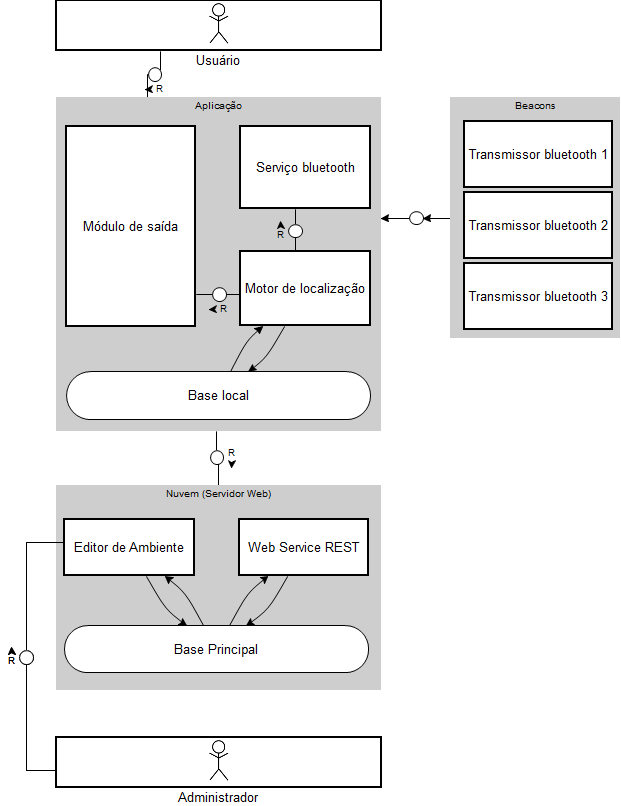
\includegraphics[width=\textwidth]{imgs/arquitetura.png}
		\fonte{Elaborado pelo autor.}
	\end{minipage}
\end{figure}

A arquitetura do modelo, bem como cada um dos componentes, é explicada em maiores detalhes nas seções subsequentes utilizando a notação Technical Architecture Modeling, ou TAM. \cite{SAPTAM}

\subsection{Cliente Insight}
O cliente Insight é projetado para ser utilizado em dispositivos móveis, fazendo uso de recursos e informações que tais aparelhos podem prover, tais como localização e portabilidade. Como pode ser observado na Figura \ref{fig:arquiteturaCliente}, o cliente é dividido em seis módulos, cada um responsável por uma parte específica da solução. Nesta subseção é detalhado o funcionamento de cada um destes módulos.

\FloatBarrier
\begin{figure}[!ht]
	\caption{Diagrama de blocos da arquitetura do cliente Insight}
	\label{fig:arquiteturaCliente}
	\centering%
	\begin{minipage}{.8\textwidth}
		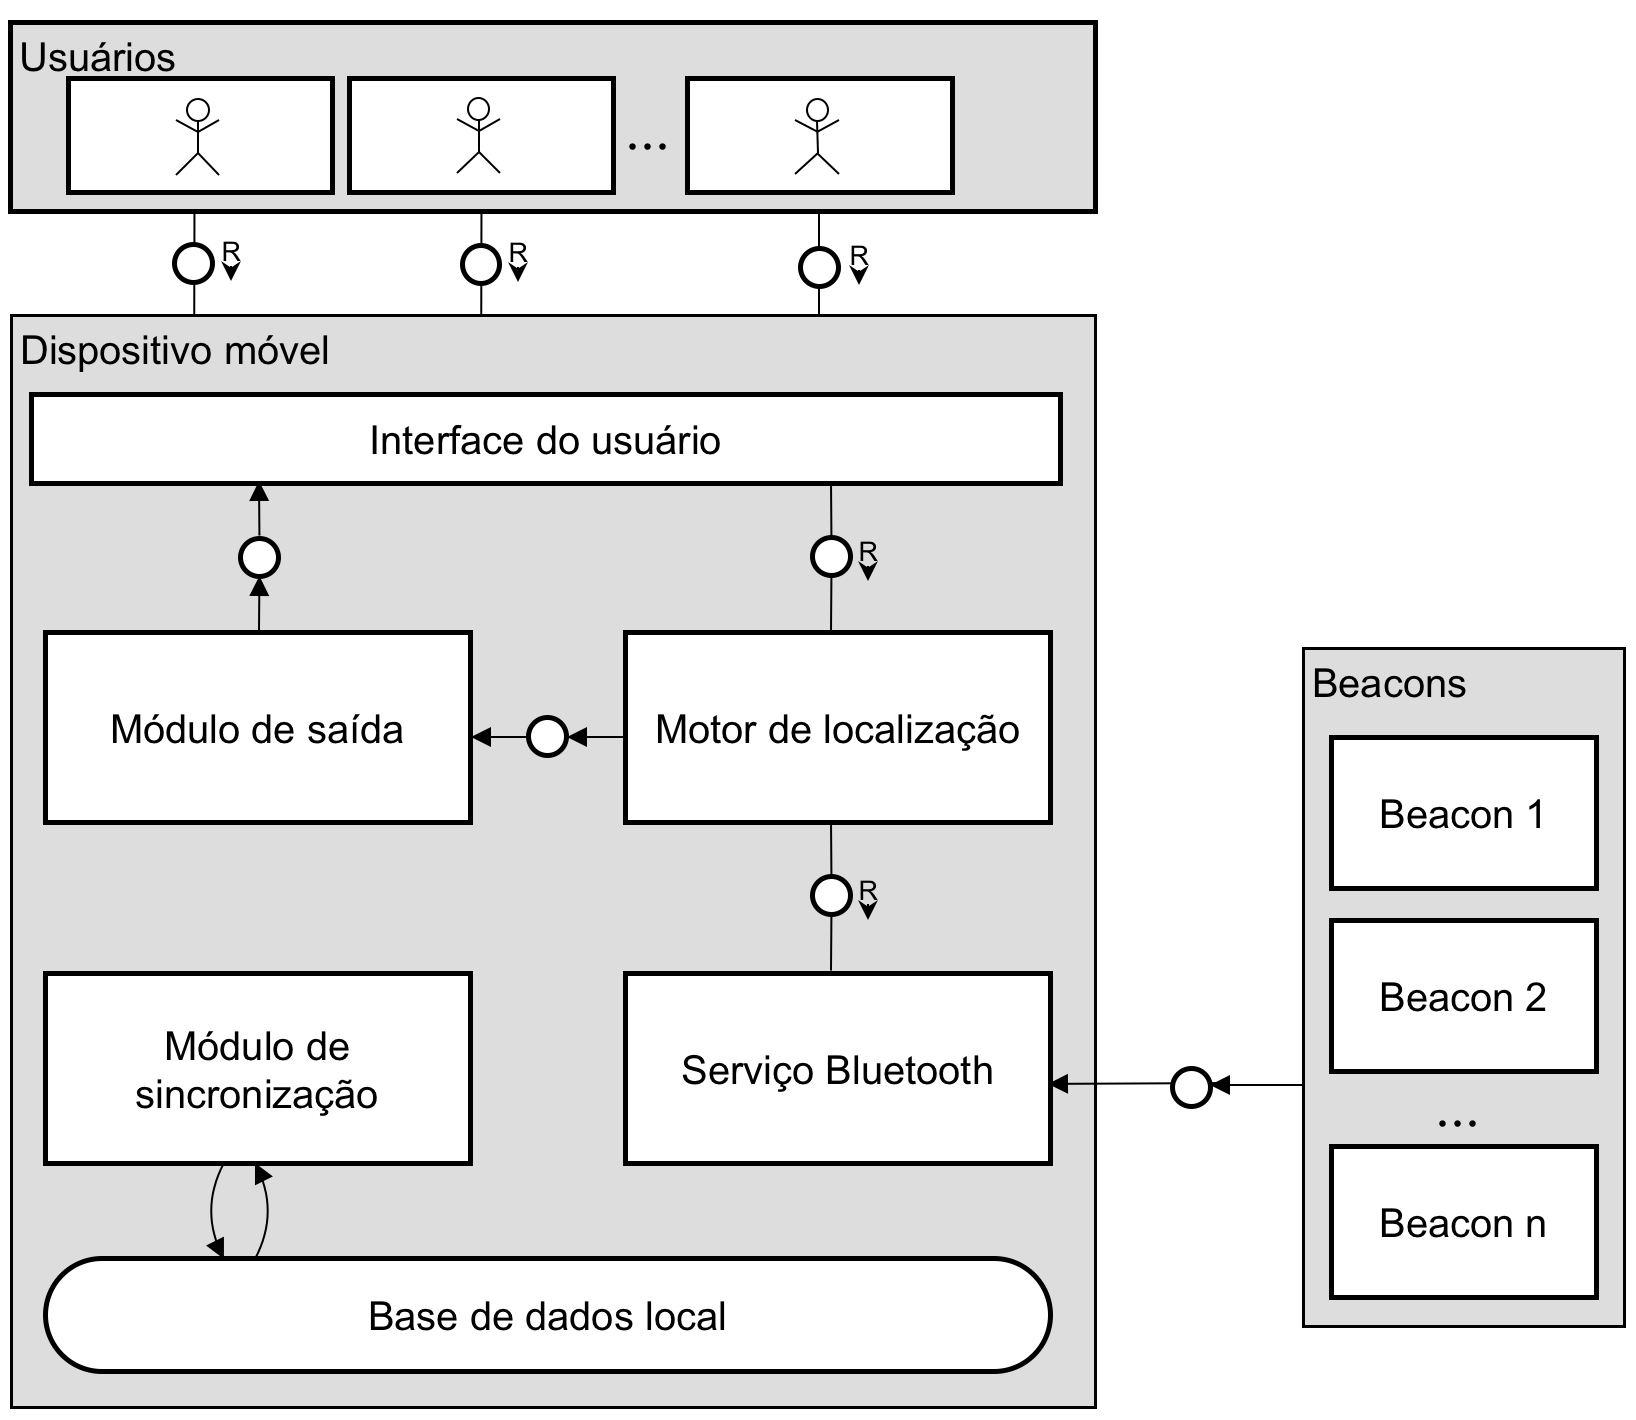
\includegraphics[width=\textwidth]{imgs/arquiteturaCliente.png}
		\fonte{Elaborado pelo autor.}
	\end{minipage}
\end{figure}
\FloatBarrier

%%%%% MODULO DE SINCRONIZACAO
O módulo de sincronização é o responsável por manter a base de dados do cliente sempre atualizada em relação a base de dados principal do modelo, afim de que o cliente possa ser utilizado sem a exigência de conexão constante com a internet. A execução da sincronização é independente do usuário, sendo feita de forma automática e transparente. Segundo \citetexto{quinones2011supporting}, uma característica muito importante em um sistema de localização acessível é a capacidade de suportar mudanças dinâmicas no ambiente, visto que caminhos já conhecidos pelos usuários podem sofrer alterações. Mudanças dinâmicas são alterações não previstas em rotas ou locais, como por exemplo um elevador não funcionando, uma sala fechada para limpeza, um caminho em manutenção, etc. Para ter tal capacidade, o período de verificação de mudanças do modelo pode ser ajustado pelo administrador.

%%%%% BASE DE DADOS LOCAL
A base de dados local tem como objetivo permitir que o cliente funcione sem exigir conexão com a internet. Ela é responsável por manter uma cópia das informações do servidor, bem como as preferências do usuário. Além disso, ela também guarda informações anônimas que visam permitir uma execução otimizada do cliente, tais como histórico de sincronização, telemetria do cliente, entre outras. A base é alimentada pelo módulo de sincronização

%%%%% MOTOR DE LOCALIZAÇÃO
O motor de localização é, juntamente com o serviço Bluetooth, o coração do Insight. Sua função é calcular a rota desde a posição atual do usuário até o destino por ele escolhido. A rota calculada pelo Insight é comunicada ao usuário de forma a se moldar à maneira com a qual os PDV planejam seu caminho, descrita por \citetexto{harper2000travel}: PDV costumam fragmentar sua jornada em partes menores e mais gerenciáveis, assim podem controlar seu deslocamento por etapas. Após ter a rota definida, o Insight a divide em trajetos menores e a comunica ao usuário em etapas. Ao terminar de percorrer um trecho, o usuário recebe as próximas instruções. De acordo com \citetexto{Falk2013}, uma definição otimizada da granularidade e da velocidade de leitura das instruções é importante para não sobrecarregar o usuário com instruções demais, podendo deixa-lo confuso e desorientado. 

Para o cálculo das rotas é usado o algoritmo proposto por \citetexto{dijkstra1959note}. O algoritmo de Dijkstra soluciona o problema do caminho de custo mínimo em um grafo cujas arestas não possuem peso negativo, como é o caso das rotas do Insight.

%%%%% SERVIÇO BLUETOOTH
O Serviço Bluetooth é a parte do Insight que faz uso da tecnologia Bluetooth Low Energy. Ele é o responsável pelo monitoramento dos beacons presentes no entorno do usuário, o que permite que sua localização possa ser determinada. Este modulo fornece o contexto do usuário para o modelo, permitindo que seja possível atuar quando mudanças são identificadas, adaptando as instruções conforme ele se aproxima ou distancia do destino. Este módulo é capaz de atuar mesmo com o smartphone no bolso do usuário, o que permite que o usuário percorra as rotas com as mãos livres e que o smartphone detecte quando o usuário adentra o ambiente onde o modelo esta instalado, avisando o usuário sobre sua existência e o questionando se ele deseja usar o cliente.

%%%%% BEACONS
Os beacons não são propriamente parte do modelo, mas é através deles que a localização do usuário é determinada. Uma vantagem da tecnologia Bluetooth Low Energy perante versões mais antigas do Bluetooth é a capacidade de transmitir e receber indicadores sem necessidade de parear os dispositivos, dispensando o usuário de qualquer ação durante o processo. Eles devem ser espalhados em pontos chave do ambiente e em todos os destinos possíveis, de forma a garantir a área de cobertura do sinal e a otimização na quantidade de beacons necessários, tornando possível para o Insight sempre descobrir a posição do usuário. O modelo não exige a posição exata e precisa do usuário, bastando apenas um beacon para fornecer a localização necessária. Caso contrario, seriam necessários três beacons por local, permitindo a triangulação da localização.

O processo de identificação de um beacon pode ser resumido como o seguinte:
\begin{itemize}
	\item Beacon transmite seu identificador no ambiente em que está instalado. 
	\item Cliente detecta a transmissão do beacon e determinar o identificador.
	\item Cliente verifica em sua base de dados a localização associada a esse identificador.
	\item Cliente obtém a localização atual do usuário e se adapta ao novo contexto.
	\item Cliente decide se há alguma ação para ser tomada, baseada no contexto do usuário.
	\item Se houver alguma ação, o cliente a executa.
	\item Cliente informa usuário sobre a ação, através de voz ou alertas vibratórios.
\end{itemize}

%%%%% INTERFACE E SAIDA
Os módulos de interface do usuário é responsável por gerenciar o trato do usuário com o sistema, enquanto o módulo de saída é responsável pelo retorno dado do usuário. Estes componentes são profundamente integrados entre si. Afim de suportar as necessidades dos PDV, a interface oferece métodos especializados de interação, como navegação por gestos e voz, enquanto o módulo de saída oferece retorno através de voz e alertas vibratórios.

Fazendo uso dos recursos acessíveis presentes nos smartphones, a interação com o sistema é drasticamente modificada de forma a facilitar o uso por parte dos PDV. \citetexto{mau2008blindaid} compara diversas formas de instruir o usuário PDV durante seu deslocamento. Após comparar instruções faladas, tons, forma de bússola e feedback tátil o trabalho indica que a melhor maneira é mesmo o uso de instruções verbais. Quando um usuário solicita que o sistema calcule uma rota até algum destino,as instruções também são passadas pelo Insight verbalmente. Porém, a leitura ocorre de uma maneira um pouco diferente. Conforme \citetexto{ullman2009accommodating}, é importante fornecer instruções claras, citando também elementos espaciais que podem ser usados como referências pelos usuários.

O Insight emite um bipe antes de cada instrução, a fim de chamar a atenção do usuário, o alertando que ele chegou em um novo marco do caminho e uma nova instrução será proferida. Instruções são passadas apenas em pontos chave do trajeto, de forma a evitar que uma frequência muito alta de informações sobrecarregue o usuário. Unidades de medidas de distância como metros são evitadas, preferindo informar o usuário do número aproximado de passos até o próximo destino. As instruções alertam o usuário sobre obstáculos no caminho, tais como escadas, aclives ou declives, caso estes existam.

Todas as falas são geradas por computador. Isso permite economizar o tamanho do software cliente, pois não é necessário armazenar arquivos de áudio, e também responder rapidamente a mudanças no ambiente, visto que não existe a exigência as falas passem por todo o processo de gravação e que o cliente tenha de ser atualizado para dispor das novas instruções.

\subsection{Componentes do serviço Insight}
O serviço Insight é o componente onde é feito o gerenciamento e monitoramento do modelo. Sua arquitetura em nuvem é projetada para oferecer escalabilidade e a tolerancia a falhas, bem como integração com outras soluções. Como pode ser visto na Figura \ref{fig:arquiteturaServico}, ela é divida em cinco módulos. Nesta subseção é detalhado o funcionamento de cada um.

\begin{figure}[!ht]
	\caption{Diagrama de blocos da arquitetura do serviço Insight}
	\label{fig:arquiteturaServico}
	\centering%
	\begin{minipage}{.7\textwidth}
		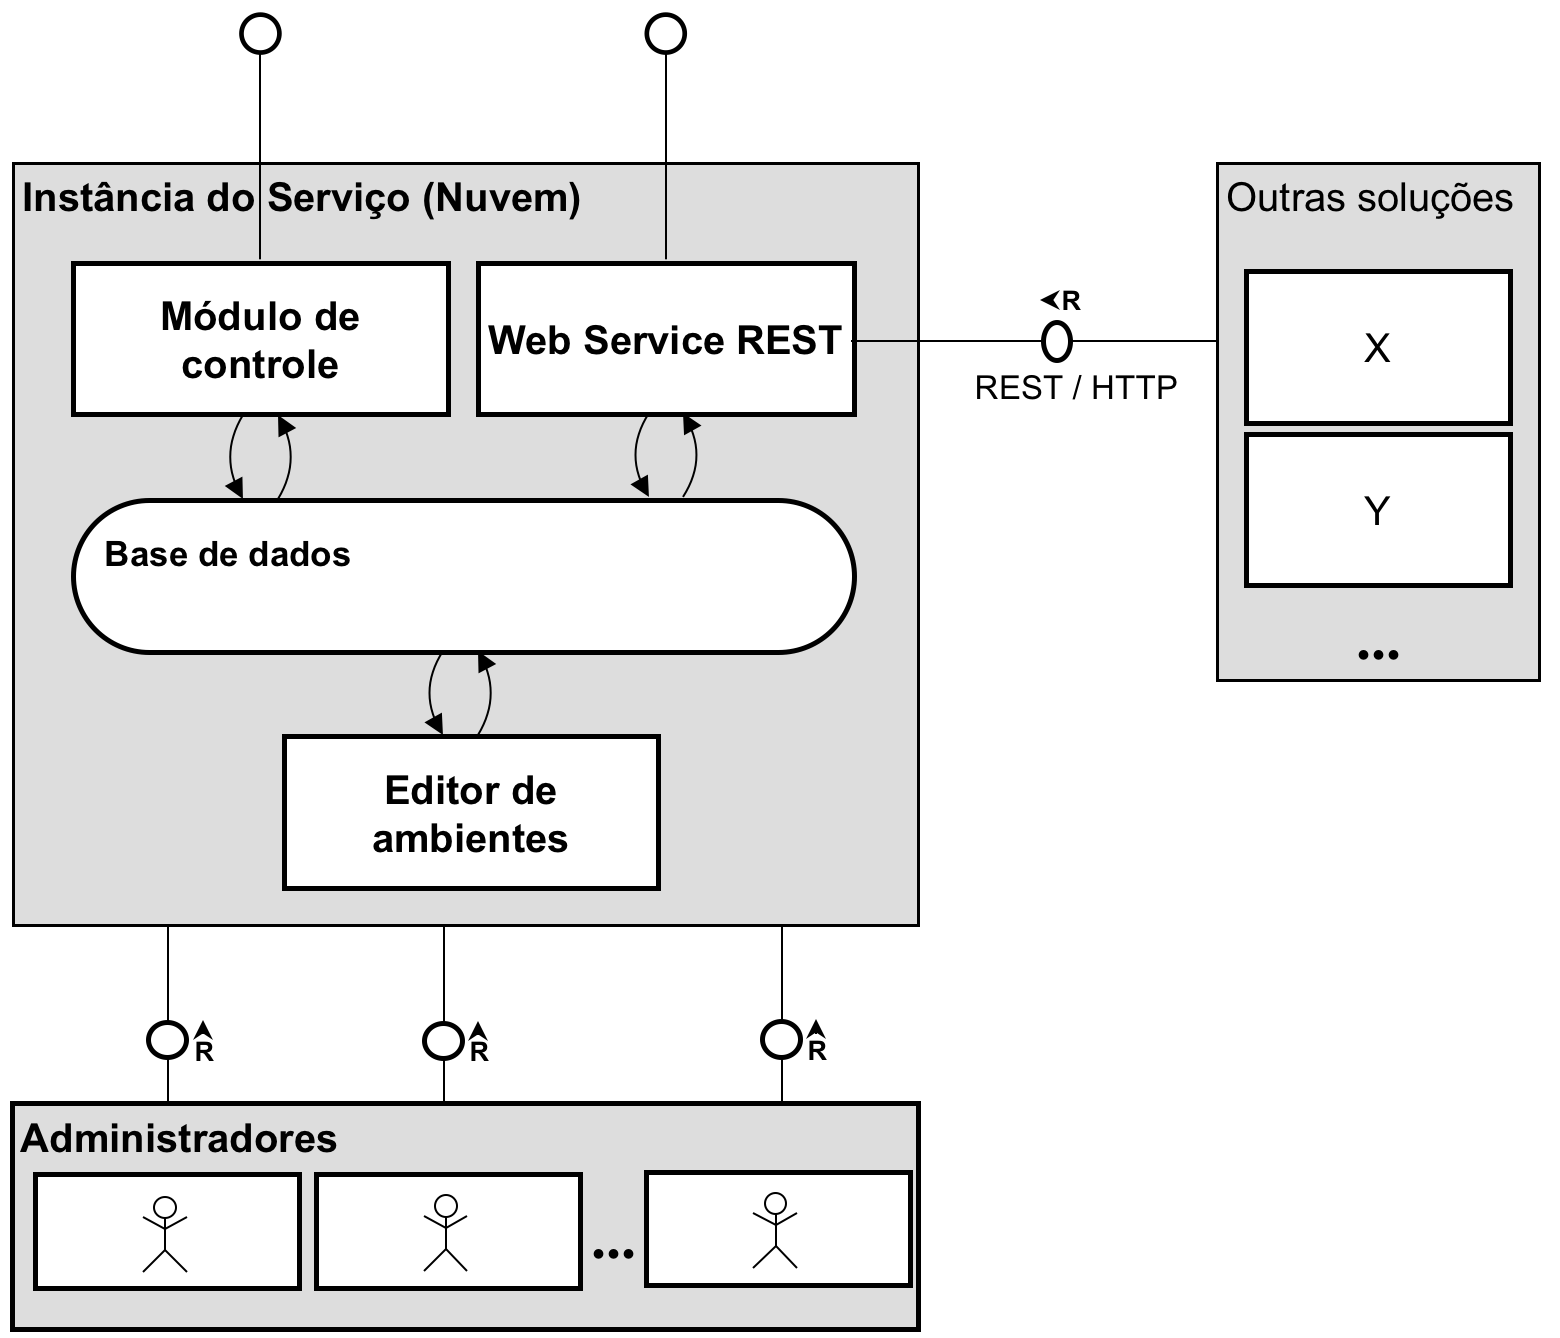
\includegraphics[width=\textwidth]{imgs/arquiteturaServico.png}
		\fonte{Elaborado pelo autor.}
	\end{minipage}
\end{figure}

O editor de ambientes é a ferramenta através da qual os administradores mapeiam o ambiente. Totalmente visual, nele os administradores criam uma representação bidimensional do ambiente, onde devem ser cadastrados os locais e recursos do ambiente, bem como trechos a serem percorridos e os locais onde estão posicionados os beacons. Para auxiliar nessa tarefa, o modelo permite visualizar áreas não cobertas pelos beacons e oferece sugestões de posicionamento.

O módulo de controle mantem informações e referências a todas as instâncias da aplicação servidor. É o responsável por gerênciar o ciclo de vida das instâncias, bem como manter seu registro de execução. Também é capaz de atuar como balanceador de carga quando detecta que uma instância está sobrecarregada, distribuindo suas requisições para outas instâncias. Este módulo oferece um painel onde podem ser monitorados em tempo real informações relevantes sobre o estado das instâncias, usuários ativos, pedidos de ajuda e outras informações analíticas.

A base de dados do serviço Insight é o principal repositório de informações do modelo. Nela ficam armazenados os beacons, rotas e locais existentes no modelo. As informações relativas os locais e rotas existentes são armazenadas em forma de grafo. Os dados aqui contidos são acessados por cada uma das instâncias através de um web service REST, assim eles podem ser acessados independentemente da plataforma utilizada.

A coleção de instâncias é o conjunto de todas as cópias da aplicação servidor sendo executadas em um dado momento. Mais detalhes sobre a aplicação servidor são apresentados na Seção \ref{componentesAplicacaoServidor}.

Um importante aspecto do modelo é sua interoperabilidade. O Insight oferece um serviço completo de localização em ambientes internos. Aliado com a infraestrutura de localização formada pelos beacons, diversas aplicações são possíveis. Cada instituição que adota o Insight pode fazer uso dos dados do modelo para desenvolver novas soluções de localização em suas dependências, aproveitando toda a infraestrutura já existente para diminuir novos custos. Os dados são expostos via web service REST, permitindo que sejam consumidos por qualquer plataforma, oferecendo flexibilidade para as soluções desenvolidas.

\subsection{Componentes da aplicação servidor}\label{componentesAplicacaoServidor}
Cada instância Insight da coleção roda uma cópia da aplicação servidor. Cada um delas é executada em um servidor físico específico, com recursos de hardware proprios, garantindo estabilidade e disponibilidade sem prejudicar a performance. Não há limite para a quantidade de instâncias executadas simultaneamente, e cada uma é independente das outras, não possuindo qualquer conhecimento sobre outras instâncias em execução. Conforme visto na Figura \ref{fig:arquiteturaInstancia}, ela é formada por três componentes, explicados em mais detalhes nesta subseção.

\begin{figure}[!ht]
	\caption{Diagrama de blocos da arquitetura da aplicação servidor}
	\label{fig:arquiteturaInstancia}
	\centering%
	\begin{minipage}{.5\textwidth}
		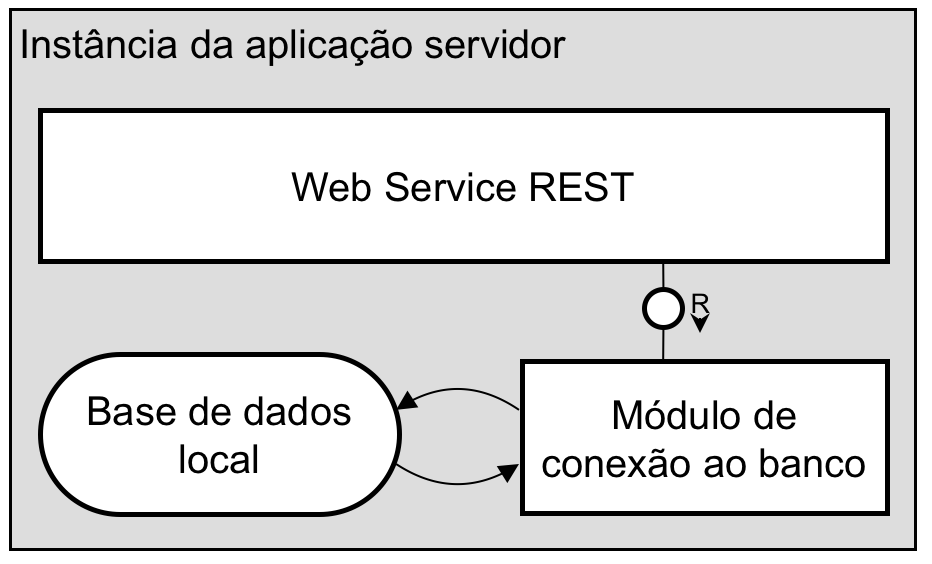
\includegraphics[width=\textwidth]{imgs/arquiteturaInstancia.png}
		\fonte{Elaborado pelo autor.}
	\end{minipage}
\end{figure}

O web service REST de cada instância é o responsável por expor os dados armazenados na base de dados. Segundo \citetexto{richardson2008restful}, REST é um padrão amplamente utilizado na comunicação entre sistemas, devido a sua capacidade de simplificar o acesso mesmo a dados bastante complexos. O padrão REST não é limitado a alguma plataforma específica, de forma que clientes em quaisquer sistemas sejam facilmente para consumir web services REST. 

Através deste componente é realizada a comunicação e a interoperabilidade do Insight. Ele recebe requisições de dados e obtem a resposta vinda do módulo de conexão ao banco. As requisições podem se originar de outras soluções ou então dos clientes Insight sincronizando dados. Os clientes Insight lidam com mudanças no ambiente consultando mais frequentemente este componente.

O módulo de conexão ao banco de dados é responsável por realizar as operações que necessitam consultar os dados cadastrados no modelo. Ele mantem registro das últimas consultas feita a base de dados, bem como os dados retornados por ela. Desta forma, quando uma nova requisição chega, ele pode determinar quem consultar, o cache da instância ou a base de dados principal do modelo.

A base de dados local da aplicação atua como um ponto de consulta intermediario entre o web service REST da instância e a base de dados principal do modelo. Ela mantem em cache uma cópia temporaria das informações que foram recentemente buscadas na base principal. Tal mecanismo tem por fim melhorar o tempo de resposta às requisições externas, uma vez que uma consulta ao cache é mais rapida do que uma consulta até a base de dados principal.

\subsection{Modelo de contexto}
No Insight, a senbilidade ao contexto do usuário é fundamental para que o modelo possa ser utilizado da forma mais intuitiva possível. Devido à natureza do modelo, a informação mais relevante é a localização do usuário. Ela será utilizada em três momentos. O primeiro é quando o usuário deseja obter uma rota até algum destino, a localização será utilizada para definir automaticamente o ponto inicial do trajeto como o ponto em que o usuário se encontra. O segundo é durante os deslocamentos, através do contexto o sistema irá automaticamente detectar a evolução do usuário no percurso definido para então fornecer o próximo conjunto de instruções, a fim dispensar qualquer tipo de interação do usuário com o modelo durante o deslocamento. O último também ocorre durante os deslocamentos pelo trajeto, com a finalidade de garantir que usuário seja avisado ao sair do trajeto determinado pelo modelo. Os três momentos oferecerão uma melhor experiência ao usuário.

Para a detecção do contexto são espalhados beacons Bluetooth pelo ambiente. Estes por sua vez emitirão sinais que serão detectados pelo smartphone do usuário ao entrar na zona de alcance do beacon. O modelo possui em seu banco de dados as informações necessárias para obter o posicionamento do beacon ao detectar seu sinal


\subsection{Implementação}
Para a avaliação do Insight foi desenvolvido um protótipo composto por alguns dos requisitos funcionais e não funcionais elencados para o modelo. O desenvolvimento foi dividido três etapas: seleção dos requisitos, escolha da tecnologia e a codificação do protótipo.

A seleção dos requisitos foi feita levando em consideração quais são considerados essenciais para uma solução completa e que seja capaz de servir como base para avaliação do modelo proposto. Os requisitos funcionais deixados de fora do protótipo são o RF03, RF10, RF11 e RF12. A listagem completa dos requisitos é encontrada no Apêndice A.

A escolha da tecnologia foi feita levando em consideração que o maior requisito do modelo é ter o cliente em um dispositivo móvel. Para atender tal requisito foram levadas em consideração as plataformas Android, iOS e Windows Phone. 

O aplicativo foi desenvolvido para a plataforma Android, escolhida por ser aquela com que o autor possui mais conhecimento e experiência. O desenvolvimento utilizou a linguagem Java, nativa desta plataforma, em conjunto com o ambiente de desenvolvimento Android Studio, pois a combinação oferece integração com as bibliotecas e funcionalidades do Android. As interfaces de usuário desenvolvidas no protótipo podem ser observadas no Apêndice B.

Durante o desenvolvimento, três modelos de smartphone com Android foram utilizados para os testes, descritos abaixo:

\begin{itemize}
\item \textbf{Samsung Galaxy Note II:} smartphone com 5,5 polegadas e resolução 1280x720, com sistema operacional Android versão 4.0
\item \textbf{Motorola Moto G:} smartphone com 5,5 polegadas e resolução 1920x1080, com sistema operacional Android versão 5.1
\item \textbf{Motorola Moto X:} smartphone com 4,5 polegadas e resolução 1280x720, com sistema operacional Android versão 5.1
\end{itemize}

\section{Avaliação}
A comunidade científica utiliza cenários para validação de sistemas sensíveis ao contexto e de sistemas ubíquos, segundo as abordagens de \citetexto{dey2001conceptual} e \citetexto{Satyanarayanan2001}, respectivamente. Seguindo estas abordagens, foram criados dois cenários para teste e avaliação do Insight. Os cenários se preocupam em simular a rotina de um usuário PDV fictício dentro de um ambiente de trabalho acessível. 

O cenário 1 apresenta a chegada do usuário a seu local de trabalho, seu deslocamento até seu posto de trabalho, sua interação com os recursos apresentados pelo modelo e o chamado por ajuda. O cenário 2 aprofunda a interação do usuário com o ambiente, mostrando seu deslocamento de seu posto de trabalho até uma das salas de reunião do prédio, passando antes por um banheiro acessível.

\subsection{Cenário 1}
\textit{Eduardo possui deficiência visual desde os 5 anos de idade. Vítima de catarata, se tornou completamente cego. Por ter perdido a visão cedo, possui lembranças limitadas sobre as poucas coisas que já viu. Algumas pessoas que nunca tiveram contato com outros PDV não sabem dar assistência a Eduardo quando ele solicita, de forma que eventualmente ele prefere não pedir ajuda a outras pessoas. Eduardo é capaz de utilizar diariamente computadores e smartphones, graças a recursos assistivos tais como leitores de tela presentes nesses aparelhos. Recentemente, Eduardo começou a trabalhar para uma empresa multinacional situada no campus da Universidade do Vale do Rio dos Sinos, graças aos recursos de acessibilidade da qual a empresa dispõe.}

\textit{Em seu primeiro dia, Eduardo já possui em seu smartphone o mais novo recurso acessível da empresa, um software chamado Insight. Conforme ele se aproxima da entrada principal da empresa, o Insight detecta sua posição e questiona Eduardo se ele deseja utilizar o aplicativo. Após resposta positiva, o aplicativo se inicia e informa a localização atual do usuário através de síntese de voz. Eduardo interage com o aplicativo de forma a selecionar o local do prédio até onde deseja ir, navegando a lista de destinos usando gestos na tela até encontrar a opção "Setor 1B". Após selecionar seu posto de trabalho, Eduardo é informado que seu trajeto será divido em oito etapas, e é instruído a seguir reto a frente para chegar até a recepção, local que marca o fim da primeira etapa. Eduardo lentamente gira em torno de seu eixo até que seu smartphone comece a vibrar, indicando a direção a seguir. Quando o telefone vibra, Eduardo inicia seu deslocamento, seguindo as instruções, até que o Insight o avise sobre sua nova localização e forneça novas instruções. Ele é instruído a virar a direta e seguir reto até passar as catracas, e assim o faz até ser avisado de que concluiu outra etapa. Ao receber as instruções do próximo caminho, Eduardo descobre que deverá subir dois lances de escada, cada um com doze degraus, para concluir a próxima etapa do trajeto. Normalmente, além da escada, existem dois elevadores a disposição, porem naquele dia eles estavam em manutenção, de forma que o Insight os evita quando calcula a rota que será informada a Eduardo. Como escadas caracterizam um trajeto perigoso, Eduardo então resolve solicitar ajuda para realizar o trajeto pela primeira vez. Para tal, Eduardo seleciona o botão Chamar Ajuda e pressiona a tela duas vezes, ativando a funcionalidade. O Insight então avisa a Eduardo que um segurança está a caminho para o ajudar. Eduardo é devidamente acompanhado até seu posto de trabalho pelo segurança.}

A tabela \ref{tab:cenario1} resume a interação entre usuário e sistema, destacando atores e ações.

\begin{table}
	\caption{Dinâmica das interações Usuário-Modelo no primeiro cenário}
	\label{tab:cenario1}
	\centering%
	\begin{minipage}{1\textwidth}
		\begin{adjustbox}{max width=\textwidth}
			\begin{tabular}{ p{1,5cm} | p{14cm} }
				\hline
			 	\textbf{Ator} & \textbf{Ação}\\
				\hline
Usuário & Com o Insight em seu smartphone, se aproxima da porta de entrada principal da empresa \\
Insight & Detecta a aproximação do usuário e pergunta ao usuário se ele deseja utilizar o aplicativo \\
Usuário & Responde positivamente \\
Insight & Detecta e informa que o usuário está na entrada principal \\
Usuário & Clica em Escolher Destino, navega a lista procurando a opção Setor 1B \\
Insight & Calcula rota até Setor 1B partindo da entrada principal, avisa que o caminho foi dividido em oito etapas e instrui o usuário a seguir reto a para chegar até a recepção, o próximo destino \\
Usuário & Gira em seu eixo para encontrar a direção em que se encontra o próximo destino \\
Insight & Vibra quando o usuário vira o smartphone na direção correta \\
Usuário & Desloca-se até a recepção seguindo as instruções \\
Insight & Detecta a nova localização do usuário e o instrui a dobrar a direita e seguir reto passando pelas catracas até o acesso ao segundo pavimento, o próximo destino \\
Usuário & Desloca-se até o acesso ao segundo pavimento, passando pelas catracas \\
Insight & Detecta nova localização e fornece as instruções até o segundo pavimento, subindo as escadas \\
Usuário & Percebe a dificuldade no percurso e decide solicitar ajuda para subir as escadas clicando no botão Chamar ajuda \\
Insight & Avisa o usuário que um segurança está a caminho \\
Usuário & Se dirige até seu posto de trabalho guiado devidamente pelo segurança. \\
				\hline
			\end{tabular}
		\end{adjustbox}
		\fonte{Elaborado pelo autor.}
	\end{minipage}
\end{table}

\subsection{Cenário 2}
\textit{É comum que em seu novo emprego, Eduardo tenha se dirigir até alguma das salas de reunião da empresa, conforme surge a necessidade. Em seu posto de trabalho, Eduardo recebe o aviso de que faltam poucos minutos até o horário de próxima reunião, de forma que ele resolve iniciar o deslocamento até o local marcado. Consultando em seu computador, Eduardo verifica que a reunião acontecerá na sala chamada 1C 01 e pega seu smartphone para iniciar o Insight. Com o telefone na mão, Eduardo desliza o dedo em sua tela até encontra o ícone do aplicativo e, assim que o faz, com um duplo toque inicia o aplicativo. Quando inicia, o Insight detecta que a comunicação Bluetooth do smartphone de Eduardo está desligada, solicitando através de voz que Eduardo a ligue afim de permitir o correto funcionamento do aplicativo. Outra vez percorrendo a tela com o dedo, Eduardo encontra opção Ativar, e com um duplo toque ativa. Uma vez que o Bluetooth esteja funcionando, o Insight detecta e informa a Eduardo sua localização atual, setor 1B. Já com o aplicativo aberto e sabendo para onde deve ir, Eduardo percebe que a reunião pode demorar e então decide passar antes no banheiro. Eduardo seleciona o botão Escolher destino e, deslizando o dedo para a direita na tela, percorre a lista procurando pelo banheiro mais próximo. Quando o encontra, com um duplo toque Eduardo o escolhe. O Insight informa que o trajeto compreendido entre seu posto de trabalho e o banheiro possui três etapas, e fornece as primeiras instruções, informando que Eduardo deve seguir em linha reta de sua posição atual até o corredor para concluir a primeira etapa. Ele gira lentamente em busca da direção correta até que o smartphone em sua mão vibre, então começa a andar. Chegando no corredor, Eduardo é informado sobre sua nova posição e o caminho que deve fazer para concluir mais uma etapa. Após encontrar a direção correta, ele segue reto até ouvir o familiar barulho da porta de correr automática que marca o fim daquela etapa, restando apenas seguir reto até que o Insight o avise que ele chegou ao banheiro.}

\textit{Prestes a sair do banheiro, Eduardo usa o Insight para obter a rota restante até a sala de reuniões 1C 01 clicando no botão Escolher destino e selecionando a opção correspondente. O novo caminho é dividido em apenas duas etapas. Obtendo as novas instruções do Insight, ele descobre que deve apenas seguir reto após sair do banheiro até que seja informado sobre a próxima etapa. Chegando ao corretor que marca a última etapa, ele deve apenas seguir até a porta em sua frente que terá chegado na sala de reuniões. O Insight detecta e informa que o usuário chegou no destino escolhido.}

A tabela \ref{tab:cenario2} resume a interação entre usuário e sistema, destacando atores e ações.

\begin{table}
	\caption{Dinâmica das interações Usuário-Modelo no segundo cenário}
	\label{tab:cenario2}
	\centering%
	\begin{minipage}{1\textwidth}
		\begin{adjustbox}{max width=\textwidth}
			\begin{tabular}{ p{1,5cm} | p{14cm} }
				\hline
			 	\textbf{Ator} & \textbf{Ação}\\
				\hline
Usuário & Inicia o Insight em seu smartphone \\
Insight & Detecta que a comunicação Bluetooth está desligada e solicita que Eduardo a ligue \\
Usuário & Liga a comunicação Bluetooth \\
Insight & Detecta e informa que o usuário está em seu posto de trabalho no setor 1B \\
Usuário & Clica em Escolher Destino, navega a lista procurando a opção Banheiro acessível 1C \\
Insight & Calcula rota até o local selecionado partindo do local atual, avisa que o caminho foi dividido em três etapas e instrui o usuário a virar para a direita de seu posto de trabalho e seguir reto até o corredor do setor, o próximo destino \\
Usuário & Gira em seu eixo para encontrar a direção em que se encontra o próximo destino \\
Insight & Vibra quando o usuário vira o smartphone na direção correta \\
Usuário & Desloca-se até o corredor seguindo as instruções \\
Insight & Detecta a nova localização e instruir o usuário a seguir reto até a porta de correr automática do setor, o próximo destino \\
Usuário & Se vira para a direita e segue reto até ouvir o som da porta \\
Insight & Instrui o usuário e passar a porta e seguir reto até o banheiro \\
Usuário & Segue reto até encontrar a porta do banheiro \\
Insight & Detecta e informa que o usuário chegou ao seu destino \\

Usuário & Prestes a sair do banheiro, clica em Escolher Destino, navegando a lista até encontrar a sala de reuniões 1C 01 \\
Insight & Calcula rota até a sala de reuniões 1C 01 partindo do banheiro, avisa que o caminho foi dividido em duas etapas e instrui o usuário a seguir reto até chegar ao corredor de acesso as salas de reunião, o próximo destino \\
Usuário & Sai do banheiro e continua seguindo reto até o corredor \\
Insight & Detecta a localização do usuário e fornece instruções até a sala de reunião 1C 01, o ultimo destino \\
Usuário & Segue reto até encontrar a sala \\
Insight & Detecta e informa que o usuário chegou ao seu destino \\
\hline
			\end{tabular}
		\end{adjustbox}
		\fonte{Elaborado pelo autor.}
	\end{minipage}
\end{table}

\subsection{Considerações}
Os cenários descritos demonstram a capacidade de localização do modelo usando como base o contexto de localização do usuário, e foram executados em ambiente controlado pelo autor deste trabalho, que o fez vendado e portando um smartphone Galaxy Note II, onde estava instalado o protótipo desenvolvido, acompanhado de um fone de ouvido simples. 

Para a localização, foram espalhados beacons Bluetooth na quantidade mínima necessária para cobertura da área de execução dos cenários na ordem descrita, cada beacon representava um local e todos foram previamente cadastrados na base do dispositivo. O protótipo foi capaz de identificar rapidamente mudanças na localização, fornecendo as novas instruções em tempo hábil.

Apenas a parte de localização, porção principal do modelo, foi testada, visto que um teste completo exigiria o desenvolvimento módulo de sincronização e do serviço na nuvem, além de outro usuário para atuar como provedor da ajuda.

Baseado no comportamento apresentado pelo protótipo... %, é possível concluir que ele atende a proposta do trabalho. Através da combinação de síntese de voz e dos recursos providos pelo modo acessível do smartphone, como leitura de tela, alertas vibratórios e navegação por gestos, foi possível prover uma experiência acessível aos usuários.


%=======================================================================
% Conclusão
%=======================================================================
\section{Conclusão}






% \section{Introdução}

% \begin{itemize}
% 	\item Cada transição de tela tem uma fala

%     //TODO: todo android vem com o sintetizador de voz
%     //TODO: inspiração veio quando minha namorada comentou que viu no trem...

%     //TODO: navigation, initicializa já no primeiro lugar do camihno
%     //TODO: app roda no plano de fundo

%         // TODO: No primeiro uso, pergunta se o usuário quer que o aplicativo monitore sua região e
%     // se auto execute quando chega na área
% \end{itemize}

%=======================================================================
% Resumo em língua estrangeira (sim, é aqui mesmo).
%
% O idioma usado aqui deve necessariamente aparecer nos parâmetros do
% \documentclass, no início do documento.
%=======================================================================
\begin{otherlanguage}{english}
\titulo{Insight: An accessible model for navigation inside indoor environments using Bluetooth Low Energy}
\begin{abstract}
Este documento apresenta orientações para uso da classe \LaTeX\ de formatação de artigos para a UNISINOS\@.  Ao mesmo tempo, ele serve como exemplo de uso da classe, demonstrando os principais comandos a serem utilizados, e outras orientações mais gerais de uso do \LaTeX.  Adicionalmente, procuramos incluir no documento algumas orientações sobre a escrita da monografia em si, reunindo dicas e recomendações que contribuem para aumentar a qualidade técnica dos trabalhos acadêmicos.  O Resumo deve conter de 150 a 250~palavras e apresentar o objetivo, o método, os resultados e as conclusões do artigo. Deve ser composto por frases concisas e afirmativas. Recomenda-se o uso de parágrafo único. Deve-se usar o verbo na voz ativa e na terceira pessoa do singular.

\palavraschave{Ubiquitous Accessibility\@.  Visual Impairment\@.  Indoor positioning systems  \LaTeX.}

\end{abstract}
\end{otherlanguage}

%=======================================================================
% Referências
%=======================================================================
\bibliography{bibliografia_artigo}


%=======================================================================
% Exemplo de Apêndice
% O Apêndice é utilizado para apresentar material complementar elaborado
% pelo próprio autor.  Deve seguir as mesmas regras de formatação do
% corpo principal do documento.
%=======================================================================
% \appendix
% \section{Requisitos}\label{apendice:requisitos}
% Este apêndice apresenta a listagem dos requisitos elicitados para o modelo Insight, sendo divididos em requisitos funcionais e não funcionais.

% \subsection{Funcionais}
% Neste apêndice são apresentados os requisitos funcionais elicitados para o modelo Insight. Cada requisito funcional corresponde a uma funcionalidade presente na modelo, a fim de que usuários possam desempenhar suas ações. Para a definição dos requisitos foi levado em consideração que o sistema possui dois tipos de atores: usuários e administradores.

% \begin{itemize}
% 	% USER
% 	\item \textbf{RF01 - Obter localização atual:} o usuário poderá obter sua localização atual a qualquer momento.
		
% 	\item \textbf{RF02 - Visualizar locais próximos:} o usuário poderá visualizar os locais próximos a si, ordenados pela distância até o local.
		
% 	\item \textbf{RF03 - Pesquisar por local:} o usuário poderá pesquisar entre os locais disponíveis usando critérios como nome ou categoria.
		
% 	\item \textbf{RF04 - Visualizar detalhes do local:} o usuário poderá visualizar informações específicas do local selecionado, tais como nome, descrição, categoria e distância até ele.

% 	\item \textbf{RF05 - Obter rota até local selecionado:} o usuário poderá obter uma rota até o local selecionado, partindo do seu local atual.

% 	\item \textbf{RF06 - Listar locais favoritos:} o usuário poderá visualizar uma lista com os locais marcados como seus favoritos.
		
% 	\item \textbf{RF07 - Manter locais favoritos:} o usuário poderá adicionar ou excluir locais da lista de locais favoritos.
		
% 	\item \textbf{RF08 - Mensagem de boas-vindas:} o sistema deverá detectar quando o usuário chega no ambiente e enviar uma notificação ao usuário perguntando se ele deseja usar o cliente.

% 	\item \textbf{RF09 - Enviar pedido de ajuda:} o usuário poderá enviar aos administradores um pedido de ajuda informando o seu último local conhecido, para que alguém seja enviado para socorrer o usuário.
		
% 	% ADMIN
% 	\item \textbf{RF10 - Manter locais:} o administrador poderá adicionar, editar, ou excluir locais e rotas cadastrados no modelo.
		
% 	\item \textbf{RF11 - Manter beacons:} o administrador poderá adicionar, editar, ou excluir beacons cadastrados no modelo.

% 	\item \textbf{RF12 - Sincronização:} o administrator poderá alterar a periodicidade das sincronizações do cliente com o servidor.
% \end{itemize}

% \subsection{Não Funcionais}
% Neste apêndice são apresentados os requisitos não funcionais elicitados para o modelo Insight. Os requisitos não funcionais descrevem aspectos internos da aplicação no que diz respeito ao desempenho, confiabilidade, interoperabilidade, mobilidade, disponibilidade, segurança e usabilidade.

% \begin{itemize}
% 	\item \textbf{RNF01 - Escalabilidade e disponibilidade - Serviço na nuvem:} A aplicação servidor será uma aplicação web.

% 	\item \textbf{RNF02 - Interoperabilidade - Serviços web REST:} a aplicação servidor disponibilizará web services utilizando o padrão Representational State Transfer (REST) para realizar a integração com os clientes e outras soluções.

% 	\item \textbf{RNF03 - Interoperabilidade - JSON:} o sistema usará o padrão Javascript Object Notation (JSON) para a transferência de informações a partir do servidor REST, a fim de facilitar a comunicação com os clientes e outras soluções.

% 	\item \textbf{RNF04 - Portabilidade - Clientes para dispositivos móveis:} a aplicação cliente será utilizado em smartphones ou tablets.

% 	\item \textbf{RNF05 - Usabilidade - Base de dados local:} O cliente deverá conter uma cópia local do banco de dados localizado na nuvem.

% 	\item \textbf{RNF06 - Confiabilidade - Sincronização:} O cliente deverá periodicamente sincronizar sua base de dados com a base de dados na nuvem.

% 	\item \textbf{RNF07 - Usabilidade - Adaptação ao contexto:} o cliente deverá identificar o contexto do usuário através do uso da localização, a fim de exibir os locais mais relevantes e fornecer os próximos passos da navegação.

% 	\item \textbf{RNF08 - Usabilidade - Comandos por gestos:} o cliente deverá permitir a interação do usuário através de gestos.

% 	\item \textbf{RNF09 - Usabilidade - Comandos por voz:} o cliente deverá permitir a interação do usuário através de comandos de voz.

% 	\item \textbf{RNF10 - Acessibilidade - Feedback por voz:} o cliente deverá fornecer informações ao usuário através do uso de voz.

% 	\item \textbf{RNF11 - Acessibilidade - Feedback tátil:} o cliente deverá fornecer informações ao usuário através do uso de alertas vibratórios.

% 	\item \textbf{RNF12 - Acessibilidade - Discrição:} o modelo deve poder ser utilizado a partir de hardware leve e discreto.

% 	\item \textbf{RNF13 - Usabilidade - Interferência:} o modelo não deve interferir em outras ferramentas que o usuário possa estar usando para se deslocar.

% 	\item \textbf{RNF14 - Confiabilidade - Cache:} cada instância deverá manter uma cópia local temporaria dos dados que forem obtidos da base principal, afim de otimizar o tempo de resposta.

% 	\item \textbf{RNF15 - Confiabilidade - Cache:} a instância deverá, a cada consulta ao banco de dados, verificar se os dados já existem na base local, antes de consultar na base principal.

% 	\item \textbf{RNF16 - Desempenho - Formato de armazenamento:} o modelo deve armazenar as informações relativas a rotas no formato de grafos.

% 	\item \textbf{RNF17 - Desempenho - Calculo de rotas:} as rotas deverão ser calculadas através do algoritmo de Dijkstra.
% \end{itemize}


% \section{Telas}
% Neste apêndice são exibidas imagens das telas que compõe a interface de usuário desenvolvidas no protótipo. As imagens mostram, em ordem, a tela inicial do sistema; a tela inicial após o sistema ter detectado a posição do usuário; a listagem de locais marcados pelo usuário como favoritos; a listagem de possíveis destinos; o aplicativo durante o deslocamento do usuário; o aplicativo após o usuário chegar ao destino escolhido.

% 	\begin{figure}[!ht]
% 		\caption{Telas do protótipo desenvolvido}
% 		\label{apendice:telas}
% 		\centering%
% 		\begin{minipage}{1\textwidth}
% 			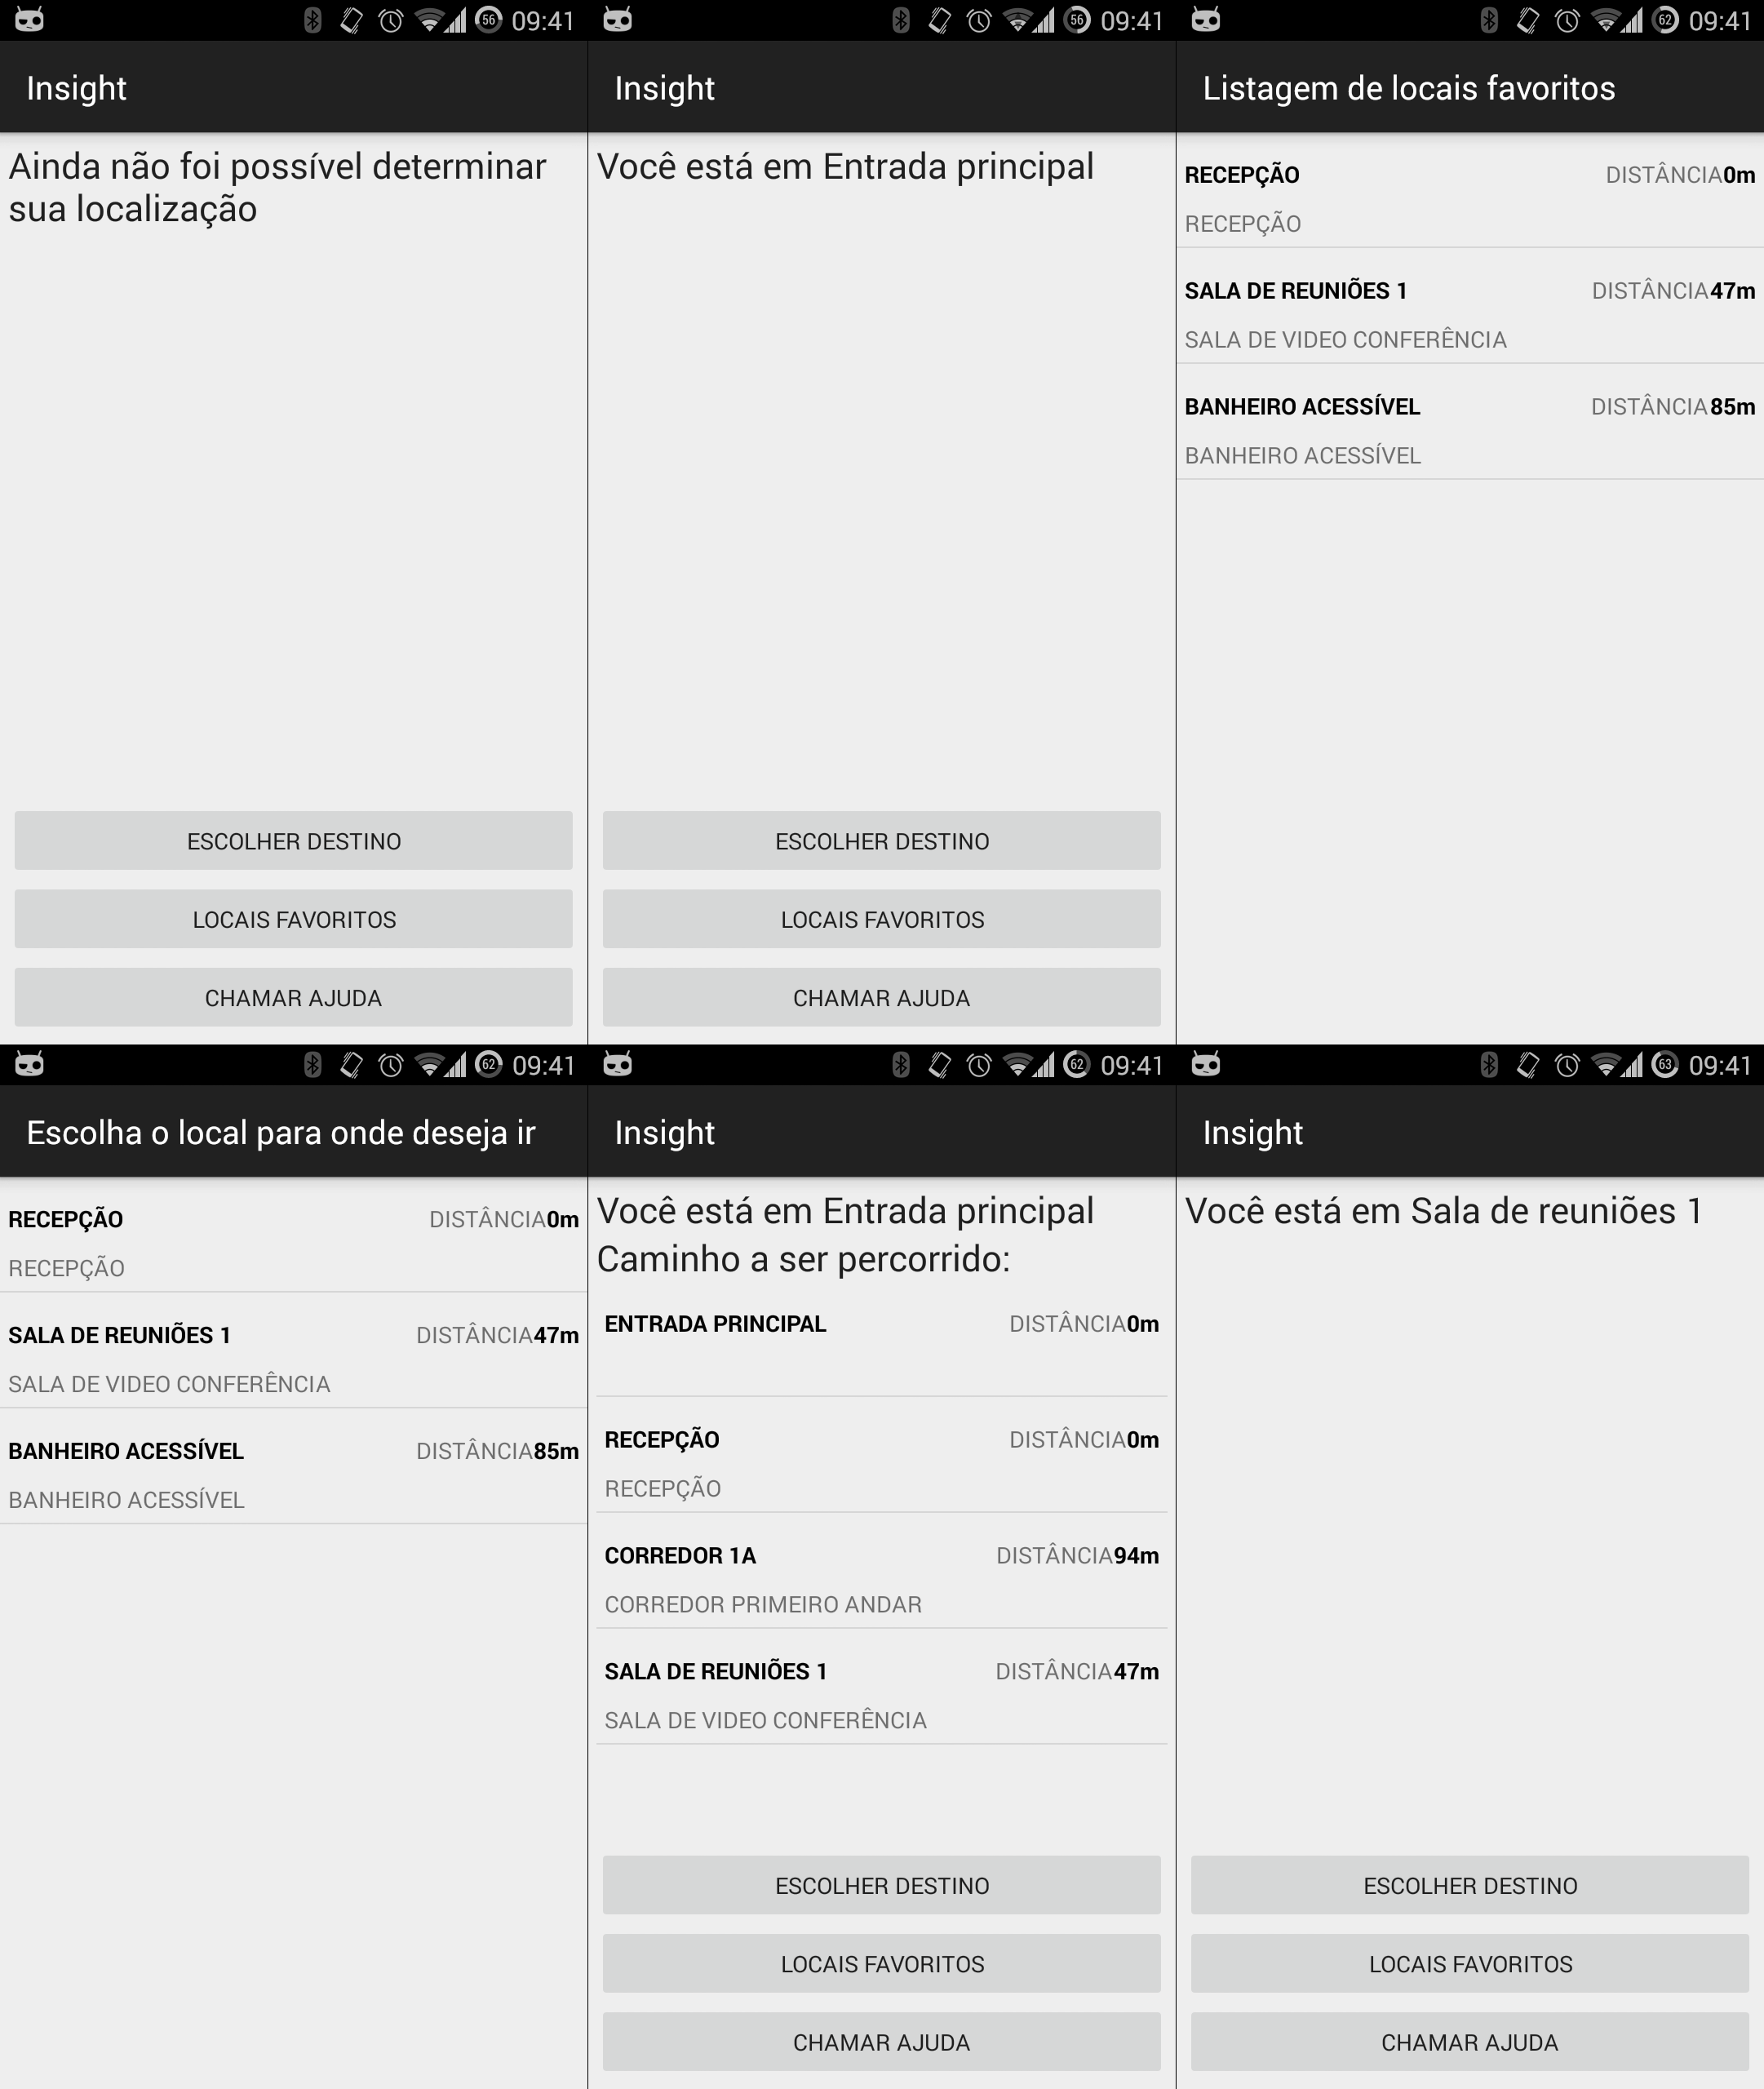
\includegraphics[width=\textwidth]{imgs/screenshots}
% 			\fonte{Elaborado pelo autor.}
% 		\end{minipage}
% 	\end{figure}

\end{document}